% TODO:
%   - Self-critical somewhere
%   - Ethical insights
%   - Surprising results - WebRTC och WebCrypto evolved during our project

Here, we lay out the outcome of the project and some of the difficulties that were met in the process. We then go through the main goals with Rymd and see how well they could be met, where and why there are shortcomings and how these could be addressed. Finally, we explore the ethical motivation behind Rymd and the implications it could have in a non-technological sense.

\section{Outcome}
This project has resulted in a modular peer-to-peer developer library for sending data, encrypted with public key encryption, over a secure connection to another client. The library, \emph{Rymd}, has composed several modules for specific areas such as data storage (section~\ref{sec:datastorage}), cryptography (section~\ref{sec:cryptography}) and communication (section~\ref{sec:p2p}) in order to create a foundation for sending files without central file storage.

For demonstrating the capabilities of Rymd, a sample prototype web application has been created, named \emph{Shuttle}. This front facing client provides a user interface for showing local files, sending files to other users registered in the blockchain, and managing encryption keys. In Shuttle the user can add, list, view and delete files in their local data store, where the files are encrypted and stored along with their metadata. By knowing a recipient's identity, the user is able to share a file with the recipient over an encrypted P2P connection. When sharing a file, the receiving end will instantly show a notification with a remark that the sender wants to share a file. If the recipient chooses to accept the sharing request, the file will be downloaded to their local data store.

\begin{figure}[ht]
\centering
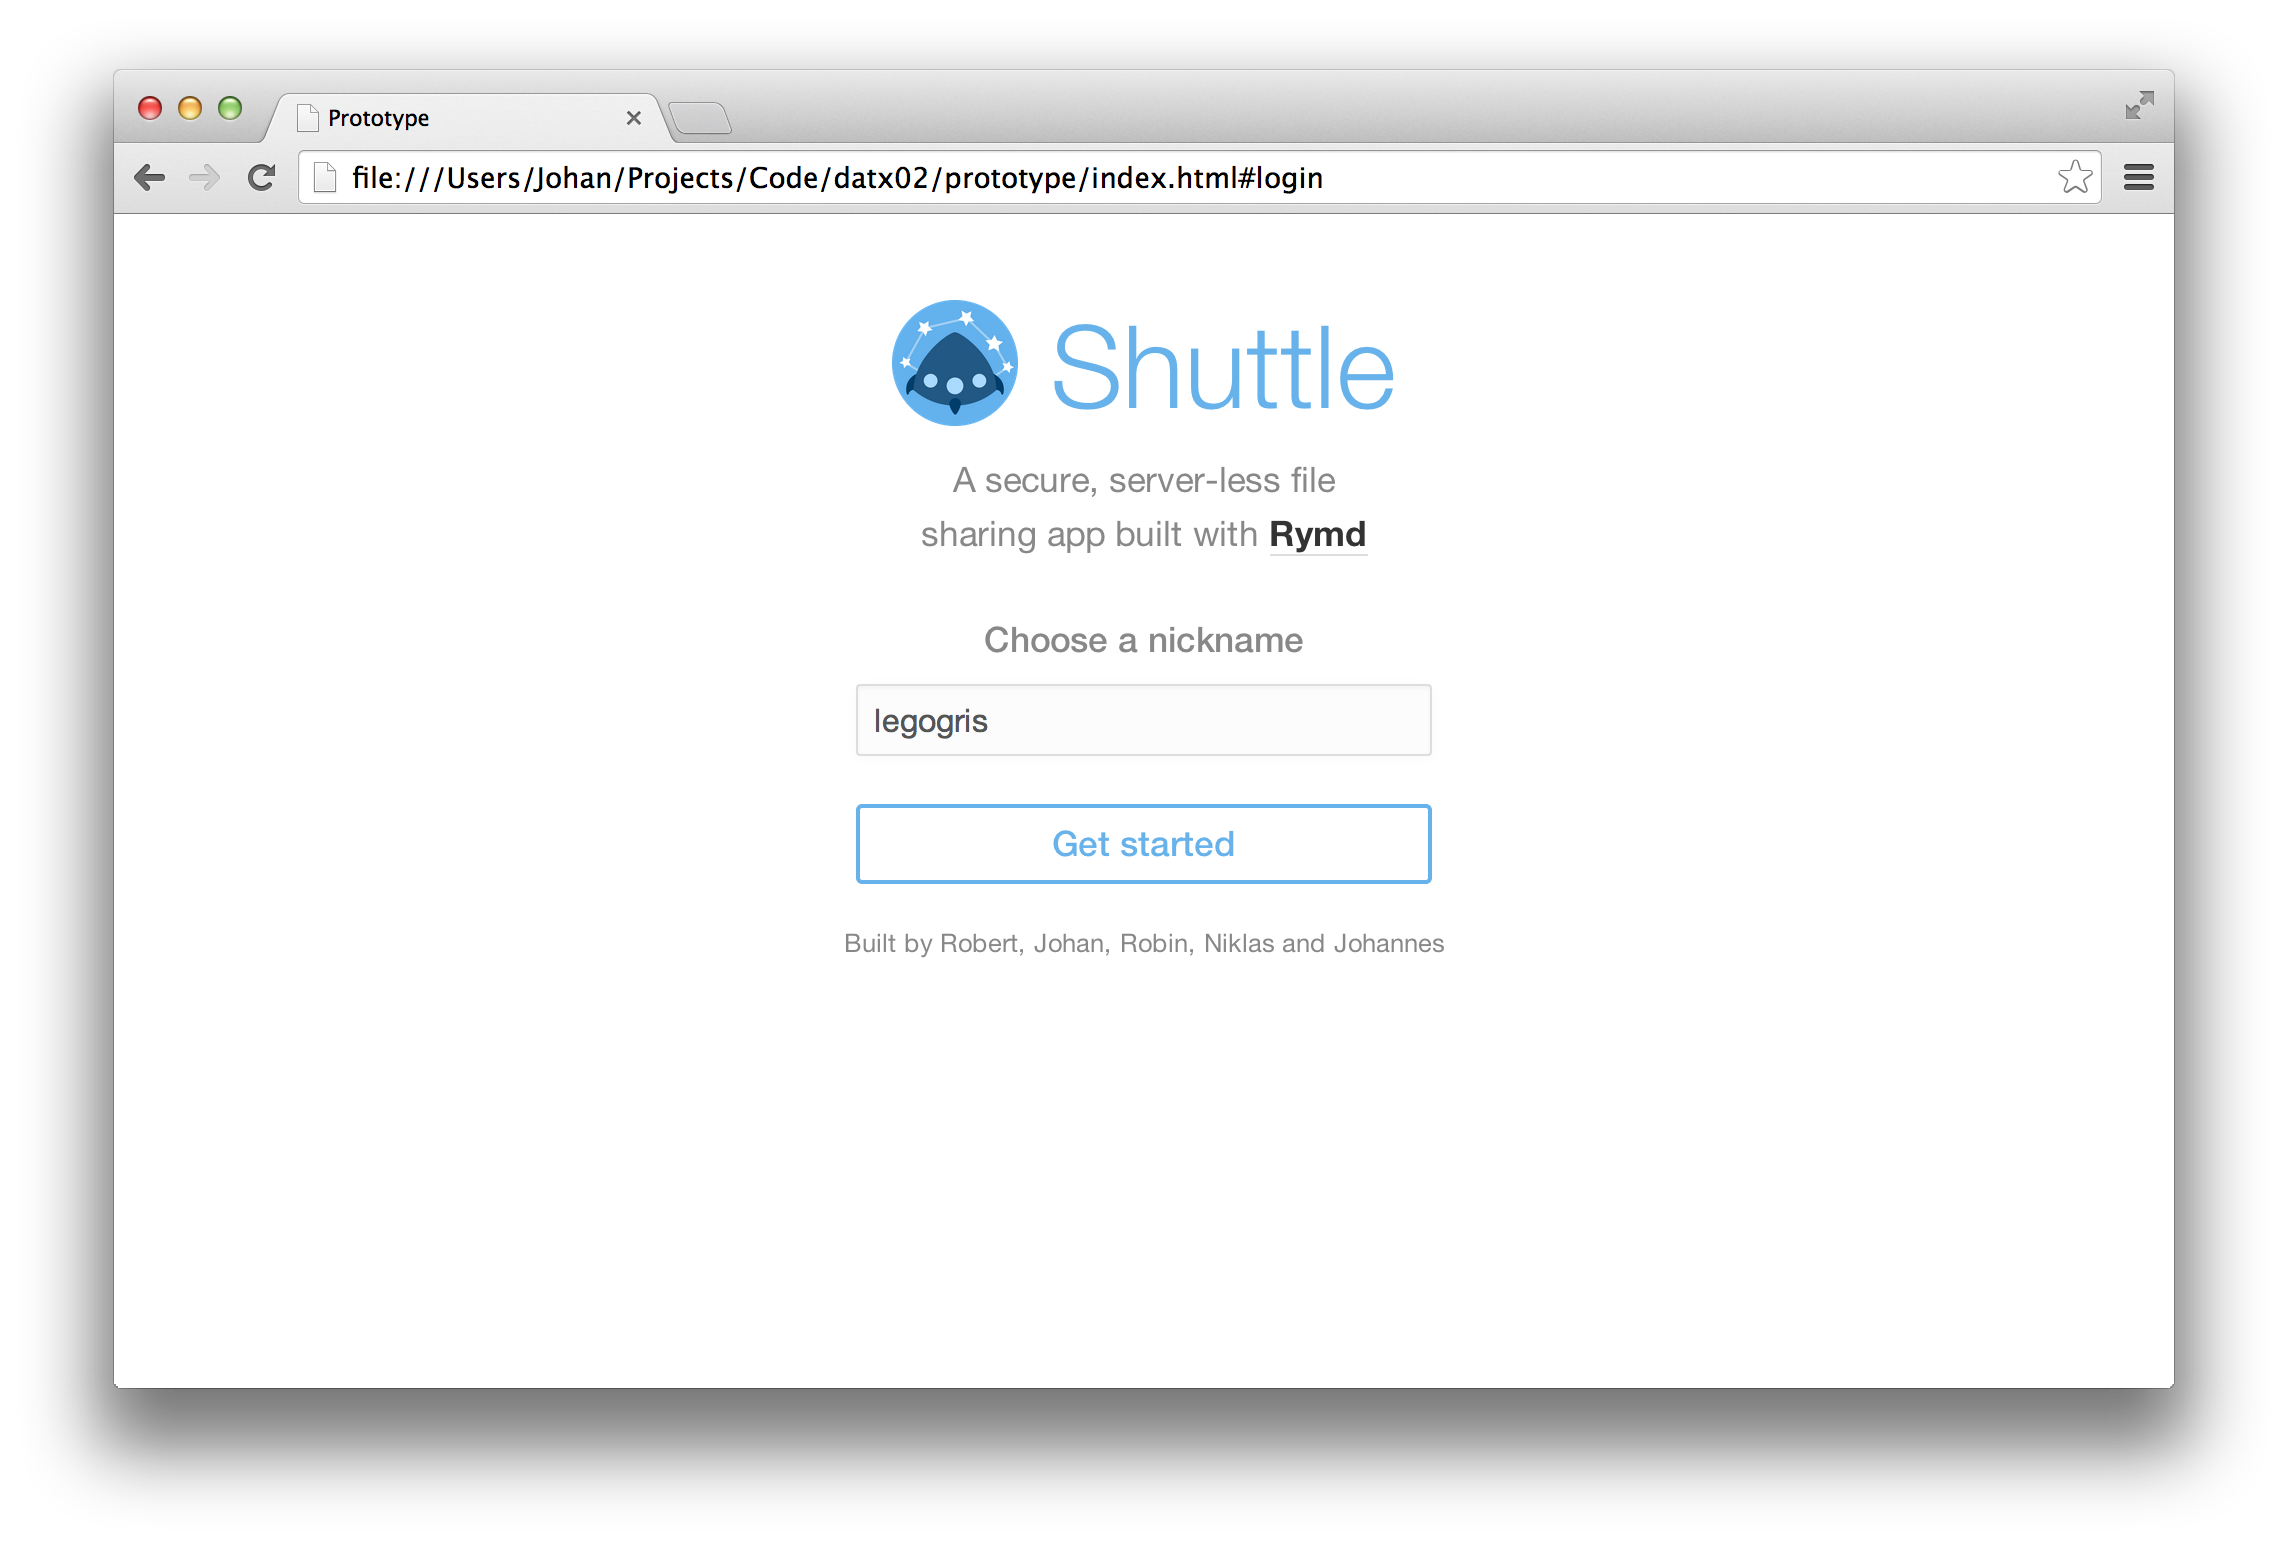
\includegraphics[width=\textwidth,height=0.2\paperheight,keepaspectratio
]{figures/shuttle-login}
\caption{The Shuttle login view}
\label{fig:shuttle-login}
\end{figure}

\begin{figure}[ht]
\centering
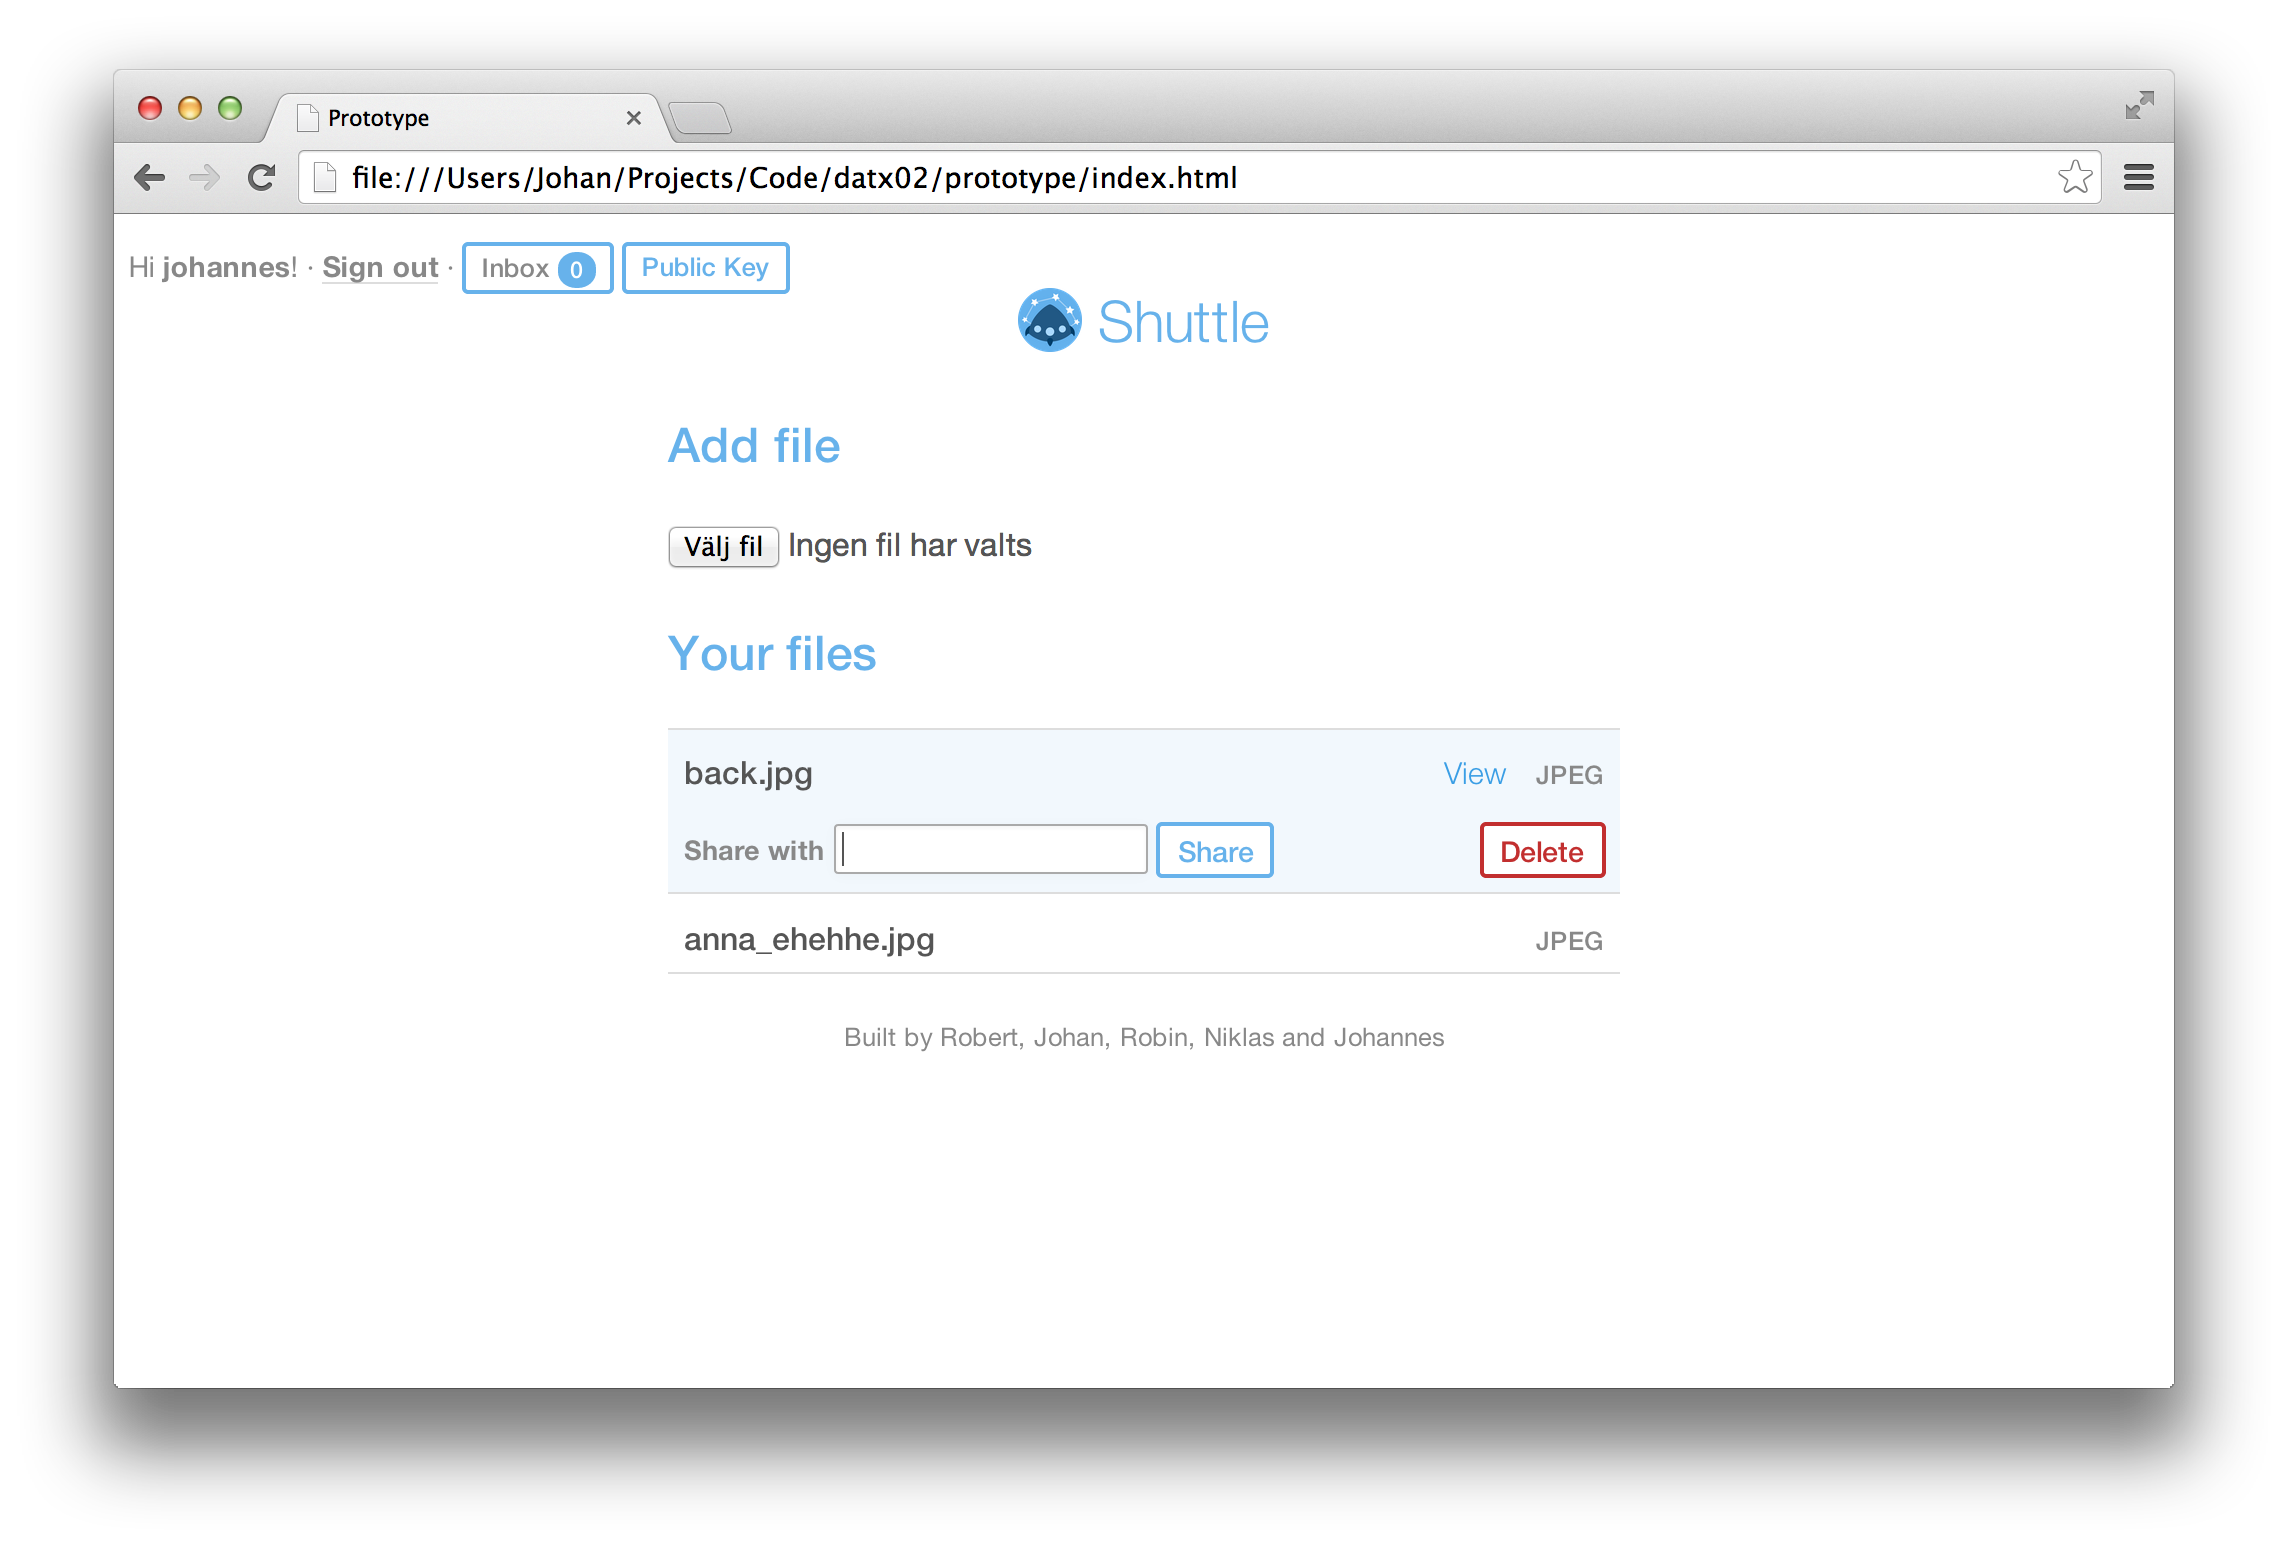
\includegraphics[width=\textwidth,height=0.2\paperheight,keepaspectratio
]{figures/shuttle-files}
\caption{Files listing in Shuttle}
\label{fig:shuttle-files}
\end{figure}

\section{A decentralized system}
One of the main initial goals for Rymd was to make the system truly decentralized and reliable independently of the availability of certain services. To a large extent, Rymd is successful in this area. Any application, including the prototype Shuttle, can be downloaded and executed locally. Therefore there are no dependencies on web servers, since all data transfers between clients are performed in a peer-to-peer fashion. No central database outside of the local client stores persistent data. There are, however, two parts where communication with central endpoints still needs to be done: connecting peers through WebRTC ICE and the interaction with the Namecoin blockchain.

\subsection{WebRTC ICE}
As described in section~\ref{sec:p2p}, establishing WebRTC connections still relies on the availability of a STUN or TURN server. This makes implementing applications depend on the availability of such a server. However, there are several public ICE servers available and in the case of downtime it is trivial to set up a new one and make the application use the new server instead. Also, since verification of identities of peers is performed locally and all data is end-to-end encrypted, there is no possibility for the administrator of these servers to spoof identities or deduce anything about shared resources. The two things that do leak are identity names (since these are needed to deduce who to connect to whom) and, if TURN is used, estimated size of data transferred. We found no way around the former and considered that the latter was a fair tradeoff - future implementations that care about leaking of resource size could solve this by also transfer redundant padding data regardless of resource size.

\subsection{Accessing the DHT}
The Namecoin blockchain is used to tie identities to their public keys and PeerJS endpoints. Therefore, an HTTP gateway running the Namecoin software was developed that acts as a bridge between the blockchain and Rymd nodes. Trust in the operator of this gateway is crucial, since public keys are fetched and verified through it. The paranoid user could, however, easily run their own gateway or manually verify or insert public keys using their own Namecoin client. In theory, each user could even run their own gateway. On May 6th, at the time of writing of this report, a public and more general HTTP/Blockchain interface at \emph{chain-api.com}\cite{Chain:2014:Online} was released. Currently it only support Bitcoin, but promises future integration with the Namecoin blockchain. Once that happens, it would be trivial to replace the current gateway with Chain if one would like to do so. The buzz around services like these shows that this is an emerging area with more interesting development to come in the near future.

Something that would both solve these issues and be very interesting in many other areas is a blockchain where nodes can communicate through open web protocols. This would mean that web clients could interact directly with the blockchain without going through external gateways like these, at the same time allowing them to contribute to the network. Given the premises stated in the introduction and the rapid development of emerging blockchains and cryptocurrencies, we think it is only a matter of time before this happens.

\section{Cryptographically secured data}
%TODO: Reference
In the application layer, all communication over WebRTC is DTLS encrypted. As stated in section~\ref{sec:creationofresources}, for local storage and sending of resources, every resource is also AES encrypted with a resource-specific key. Since all existing browser implementations of the Web Cryptography API are still experimental and partial, and there is not yet support for secure storage of cryptographic keys, the keys are stored alongside their encrypted data in IndexedDB. As long as the keys are not passphrase protected, this effectively means that at the level of the local client, the encryption adds no extra protection and can be considered redundant. An adversary gaining access to the database with the encrypted data would also have access to the decryption key. When the WebCrypto Key Discovery API becomes finalized and implemented across browsers, separate key storage options will become available and can be implemented in Rymd.

Despite this problem, the AES encryption still serves a purpose. Consider an application utilizing Rymd where users communicate through each other in a \emph{darknet} fashion - anonymous file sharing where peers are only connected to peers they trust, but data is relayed through chains of connections to facilitate propagation of data. In these cases it is imperative that resources can be transmitted separately from their keys and metadata so that intermediate peers can relay the transfer of resource data without gaining knowledge of the contents.

Also, systems with updateable resources can and should regenerate keys for each version and backward secrecy - the property that access to the key for one version of the resource will not allow decryption of older versions of that resource - will be achieved.

\section{A modular and implementation agnostic system}
As much of Rymd uses and relies on some of the latest web technologies, great care was taken during development to not make it rely on any of these implementations, should they be superceded or complemented by other more fitting alternatives. The main Rymd library itself handles only the business logic of the system and gets the modules implementing data storage, cryptography, peer-to-peer communication and DHT interaction supplied at runtime via dependency injection. Developers who have their own idea of how these needs should be served in their ownprojects could write their own implementation modules. The one area where work needs to be done is that currently, storage of keys, metadata and resource data are tied together. Before Rymd can go stable, this should be addressed by treating these as separate data stores altogether even if the current implementation puts all three side by side in IndexedDB.

Furthermore, a system with separate interchangeable parts allowed for both advantages and disadvantages. Easier testing was one of the former, where instead of a suite covering the whole system, tests could be limited to each module. Something that proved to be more difficult was the debugging of events that flow through multiple modules. Data would travel through connecting endpoints between modules and then be sent far down call hierarchies (perhaps triggering new events or having more information appended to it) before bubbling back up in the call chain. Any error occuring in such a flow were hard to pinpoint.

\section{Trusting a distributed web based application}
Currently, major web browsers have no way to verify client-side code for web applications the way that native binaries or Java applets can be cryptographically verified using signatures. Since system logic is run in a web browser, users can not know for sure whether the client code is altered between executions or not. This issue is one of the reasons why a large part of the online community is considering client-side JavaScript encryption to be a generally bad practice \cite{Matasano:Online}. If the application is delivered in form of a web browser extension, it can be signed using a certificate. This means, however, that the application has to be specifically bundled for each web browser which limits the practical portability of the code. These extensions are currently mainly available for desktop browsers. In the case of Rymd, it all depends on how the developers of implementing applications uses it.

\section{Ethical aspects}
Rymd was originally conceived from an ethical issue: that free, private and secret communication should be easily accessible and usable on the web. As it currently stands, truly secret and private communication requires running binary files and/or putting trust in a service provider. Rymd aims to be a step away from that restriction.

At its current state, Rymd should not be trusted with confidential data. This is mainly because of the limitations stated in the preceding sections that come from the choice of still immature, cutting-edge technnologies. Also, Rymd is still in an experimental stage and should not be considered stable or trusted until it has been exposed to extensive peer review and scrutiny by the community - a reservation that applies for any project of this nature. However, we are confident that we are going in the right direction and hope that further development could make Rymd a contributor in the movement of free communication on the web.

\subsection{Implications}
As always when it comes to services enabling private communication, concerns are raised on the issue of what they can be used for. Commonly mentioned are terrorism, drug dealing and child pornography. First, we want to emphasize that Rymd does not in itself provide any anonymity for its users (though it could easily be used in conjunction with anonymization services such as TOR\footnote{https://www.torproject.org}). While Rymd could indeed be used for these purposes, there are already other services such as those mentioned in section~\ref{chap:similar} that are currenly used for these purposes - Rymd does not enable risks that are not already present.

Inevitably, the question of whom is to hold responsible for malicious activity is raised when a project of this nature is realized. Some argue that developers can be held responsible since they are enabling this behaviour with less risk of repercussions. Others argue that as long as surveillance and data mining are increasingly abused by authorities and private organizations over the world, the access to private and secret communication is becoming ever more important. Technology exploring new frontiers is always met with a critical gaze; laws and regulations have merely briefly halted advancement. One way or other, technological evolution has always prevailed once the genie is out of the bottle.

Most importantly, however, it is our opinion that private and secure communication without corporation or government surveillance is a human right, and this right is effectively nonexistant if it requires significant monetary resources and/or technical know-how. Putting this standpoint aside, we have mainly treated this issue as a technical one and will let the readers of this report decide for themselves where they stand and how Rymd relates to this.
